\documentclass[conference]{IEEEtran}
\usepackage{cite}
\usepackage{amsmath,amssymb,amsfonts}
\usepackage{algorithmic}
\usepackage{graphicx}
\usepackage{textcomp}
\usepackage{xcolor}
\usepackage{float}
\usepackage{tikz}
\usetikzlibrary{positioning, shapes.geometric}
\usepackage{url}
\usepackage{subcaption}
\usepackage[compatibility=false]{caption}
\usepackage{array,tabularx,booktabs}
\usepackage{siunitx}
\usepackage{ragged2e}
\usepackage{etoolbox}
\usepackage{enumitem}
\usepackage{makecell}
\usepackage{multirow}
\usepackage{pifont}
\usepackage{listings}
\usepackage{comment}

% IEEE compliance fixes
\makeatletter
\patchcmd{\@maketitle}{\par}{\vspace*{-2ex}\par}{}{}
\makeatother

% Custom commands
\newcommand{\cmark}{\ding{51}}% ✓
\newcommand{\xmark}{\ding{55}}% ✗

% SI unit configuration
\sisetup{
 per-mode = symbol,
 group-digits = integer,
 output-decimal-marker = {.}
}

% Table formatting
\newcolumntype{Y}{>{\RaggedRight\arraybackslash}X}
\renewcommand{\arraystretch}{1.2}
\captionsetup[table]{font=small, labelfont=bf}
\setlist[itemize]{noitemsep, topsep=2pt}

% Code listing style
\definecolor{codegreen}{rgb}{0,0.6,0}
\definecolor{codegray}{rgb}{0.5,0.5,0.5}
\definecolor{codepurple}{rgb}{0.58,0,0.82}
\definecolor{backcolour}{rgb}{0.95,0.95,0.92}

\lstdefinestyle{mystyle}{
    backgroundcolor=\color{backcolour},
    commentstyle=\color{codegreen},
    keywordstyle=\color{magenta},
    numberstyle=\tiny\color{codegray},
    stringstyle=\color{codepurple},
    basicstyle=\ttfamily\footnotesize,
    breakatwhitespace=false,
    breaklines=true,
    captionpos=b,
    keepspaces=true,
    numbers=left,
    numbersep=5pt,
    showspaces=false,
    showstringspaces=false,
    showtabs=false,
    tabsize=2
}
\lstset{style=mystyle}

\begin{document}

\title{LoRA Fine-Tuning for Next User Turn Prediction in Multi-Turn Dialogues}

\author{
\IEEEauthorblockN{Sebastian Boehler\IEEEauthorrefmark{1} and Tianxiang Lu\IEEEauthorrefmark{1}}
\IEEEauthorblockA{\IEEEauthorrefmark{1}IU International University of Applied Science, Juri-Gagarin-Ring 152, 99084 Erfurt, Germany \\
Email: sebastian.boehler@iu-study.org, tianxiang.lu@iu.org}
}
\maketitle

\begin{abstract}
Most dialogue research optimizes assistant responses, leaving user-turn prediction underexplored. We investigate QLoRA fine-tuning of four open-source instruction-tuned LLMs (1.2B--7B parameters) for generating the next user utterance in multi-turn conversations. Models are trained on 6{,}000 samples from two complementary corpora, open-domain (WildChat) and task-oriented (Schema-Guided Dialog), and evaluated against unfine-tuned baselines and GPT-4o-mini prompt baselines using perplexity, BERTScore, BLEURT, and a blinded human study of 369 samples. Fine-tuning consistently improves fluency and semantic quality across three of four model families, with Llama-3B achieving the highest automated scores (0.854 BERTScore, 0.393 BLEURT). Human evaluation confirms a +0.34 average improvement on a 5-point scale, with task-oriented dialogue benefiting more (+0.45) than open-domain conversation (+0.21). A systematic ablation of 56 experiments identifies the optimal LoRA configuration. Our results demonstrate that parameter-efficient fine-tuning is a practical and reproducible approach for user-turn prediction on a single GPU.
\end{abstract}

\begin{IEEEkeywords}
Large Language Models, LoRA, Fine-tuning, Dialogue Systems, User Turn Prediction
\end{IEEEkeywords}

\section{Introduction}

Conversational AI has progressed from rule-based systems to end-to-end generative models built on the transformer architecture~\cite{vaswani2017attention, serban2016hierarchical}. The vast majority of this research focuses on improving the \emph{assistant's} response quality, while user behavior is typically modeled with hand-crafted templates or reinforcement-learning agents~\cite{shi2019simulators}. This imbalance limits the realism of dialogue evaluation and the ability to stress-test systems against diverse user behavior.

Predicting the next user turn is inherently more challenging than generating assistant responses: user utterances are less constrained, span a wider range of intents, and depend heavily on conversational context. Naous et al.~\cite{naous2025flipping} recently demonstrated that assistant-trained LLMs make poor user simulators, with the counterintuitive finding that stronger assistants produce worse user simulations. Accurate generative user modeling would enable realistic dialogue simulation, continuous system evaluation, and stress testing without requiring human participants.

In this paper, we investigate QLoRA fine-tuning~\cite{dettmers2023qlora} of four open-source instruction-tuned LLMs (1.2B--7B parameters) for next user turn prediction. We train on 6{,}000 samples drawn equally from an open-domain corpus (WildChat~\cite{zhao2024wildchat}) and a task-oriented corpus (Schema-Guided Dialog~\cite{rastogi2020sgd}), and compare against unfine-tuned base models and GPT-4o-mini zero-shot and few-shot prompt baselines.

Our contributions are as follows:
\begin{enumerate}
    \item A multi-model QLoRA study for generative user-turn prediction, evaluating four architectures across open-domain and task-oriented dialogue.
    \item A systematic two-stage ablation of LoRA hyperparameters comprising 56 experiments.
    \item A combined evaluation using three automated metrics and a blinded human study of 369 samples.
    \item Evidence that fine-tuning yields substantially larger gains on task-oriented dialogue than on open-domain conversation.
\end{enumerate}

The remainder of this paper is organized as follows. Section~II reviews related work. Section~III describes our methodology. Section~IV details the experimental setup. Section~V presents results. Section~VI discusses findings and limitations. Section~VII concludes.

\section{Related Work}

\subsection{User Simulation and Turn Prediction}

User simulators have traditionally relied on rule-based or agenda-based architectures for training reinforcement-learning dialogue policies~\cite{shi2019simulators}. Neural approaches extended this paradigm: Kim and Lipani~\cite{kim2022multitask} proposed a multi-task model that jointly predicts user actions, satisfaction, and utterances in goal-oriented settings, while Lin et al.~\cite{lin2022gentus} introduced GenTUS, a generative transformer that produces both semantic actions and natural language for task-oriented user simulation. More recently, Yoon et al.~\cite{yoon2024evaluating} evaluated LLMs as generative user simulators for conversational recommendation, finding discrepancies between simulated and real user behavior including low item diversity and incoherent feedback. The most closely related work is Naous et al.~\cite{naous2025flipping}, who introduced purpose-built \emph{User Language Models} and demonstrated that assistant-trained LLMs make poor user simulators, with the surprising finding that better assistants yield worse simulators. Their approach uses full-parameter fine-tuning of base-model checkpoints on over one million WildChat samples, conditioned on GPT-4o-generated intent summaries, requiring 227 GPU-hours on four A6000s. Our work differs in several key respects: we use QLoRA~\cite{dettmers2023qlora} on instruction-tuned models with only 6{,}000 training samples and no intent conditioning; the model learns to predict the next user turn solely from conversation history. This makes our approach substantially more resource-efficient while also enabling cross-domain evaluation across open-domain and task-oriented dialogue with four model families ranging from 1.2B to 7B parameters.

\subsection{Parameter-Efficient Fine-Tuning}

Full fine-tuning of large language models is prohibitively expensive for many research settings, motivating parameter-efficient alternatives. LoRA~\cite{hu2021lora} freezes pretrained weights and injects trainable low-rank decomposition matrices into transformer layers, reducing trainable parameters by over 99\% while matching full fine-tuning quality. The key insight is that weight updates during adaptation reside on a low intrinsic dimension, so very low ranks suffice. QLoRA~\cite{dettmers2023qlora} extends this by quantizing the frozen model to 4-bit precision and introducing paged optimizers for memory spikes, enabling fine-tuning of models up to 65B parameters on a single 48\,GB GPU. These methods are particularly relevant for our setting: they allow controlled study of behavioral adaptation, i.e., shifting a model from assistant-style to user-style generation, without full retraining, and they make the experiments reproducible on academic hardware.

\subsection{Evaluation of Generated Dialogue}

Evaluating generated dialogue remains an open challenge. Liu et al.~\cite{liu2017hownoteval} showed that word-overlap metrics such as BLEU correlate weakly with human judgments for dialogue, motivating learned alternatives. BERTScore~\cite{zhang2020bertscore} computes token-level cosine similarity using contextual embeddings, capturing paraphrases and synonyms that surface-level metrics miss; the authors recommend the F1 variant for its reliability across settings. BLEURT~\cite{sellam2020bleurt} is a learned metric pre-trained on synthetic perturbations and fine-tuned on human ratings, offering robustness to distribution shifts between training and evaluation domains. Perplexity complements these semantic metrics by measuring token-level predictability, reflecting fluency rather than meaning. Since no single automated metric fully captures conversational plausibility, we combine all three with a blinded human evaluation covering relevance, coherence, and naturalness on a 1--5 Likert scale.

\section{Methodology}

\subsection{Task Definition}

Given a multi-turn conversation history $C = (u_1, a_1, u_2, a_2, \ldots, a_{t-1})$ between a user and an assistant, the task is to generate the next user utterance $\hat{u}_t$. We frame this as a conditional language generation problem: the model receives the full context $C$ formatted as a chat template and produces $\hat{u}_t$ autoregressively. During training, only the tokens of the target user turn are supervised; all context tokens are masked (label $= -100$). This formulation differs from standard assistant modeling: user turns are typically shorter, lack the instructional structure of assistant responses, and span a wider range of communicative intents, ranging from terse confirmations to complex multi-part requests.

\subsection{Datasets}

We use two complementary datasets to evaluate cross-domain generalization. \textbf{WildChat-1M}~\cite{zhao2024wildchat} contains one million real user--ChatGPT conversations spanning diverse topics and languages; we filter for English, multi-turn ($\geq$3 turns) dialogues ending with an assistant turn, yielding context--target pairs where the target is the penultimate user utterance. \textbf{Schema-Guided Dialog} (SGD)~\cite{rastogi2020sgd} provides over 16k task-oriented dialogues across 16 service domains with structured intents. We sample 3{,}000 training and 200 evaluation pairs from each dataset (Table~\ref{tab:dataset}), interleaved for balanced domain representation, with a fixed seed of 42.

\begin{table}[h]
\centering
\caption{Dataset Statistics}
\label{tab:dataset}
\begin{tabular}{lrrr}
\toprule
\textbf{Dataset} & \textbf{Train} & \textbf{Eval} & \textbf{Total} \\
\midrule
WildChat-1M & 3,000 & 200 & 3,200 \\
Schema-Guided Dialog & 3,000 & 200 & 3,200 \\
\midrule
\textbf{Total} & 6,000 & 400 & 6,400 \\
\bottomrule
\end{tabular}
\end{table}

\subsection{Models}

We evaluate four open-source instruction-tuned LLMs spanning 1.2B to 7B parameters (Table~\ref{tab:models}), selected to test whether LoRA-based user-turn adaptation generalizes across architectures and model scales. All models use chat-template formatting with system, user, and assistant roles. As a prompt-only baseline, we include GPT-4o-mini in zero-shot and few-shot (3 exemplars) configurations, queried via API at temperature 0.4 with a maximum of 256 tokens.

\begin{table}[h]
\centering
\caption{Models Evaluated}
\label{tab:models}
\begin{tabular}{ll}
\toprule
\textbf{Model} & \textbf{Parameters} \\
\midrule
Qwen2.5-3B-Instruct & 3B \\
Llama-3.2-3B-Instruct & 3B \\
OLMo-3-7B-Instruct & 7B \\
LFM2.5-1.2B-Instruct & 1.2B \\
\midrule
GPT-4o-mini (prompt baseline) & -- \\
\bottomrule
\end{tabular}
\end{table}

\subsection{Training Setup}

All models are trained with QLoRA~\cite{dettmers2023qlora}: base weights are quantized to 4-bit NormalFloat with bfloat16 compute dtype, and only the injected LoRA adapters are updated. We use the paged AdamW 8-bit optimizer with a cosine learning rate schedule, gradient checkpointing, and a maximum context length of 4{,}096 tokens. The effective batch size is 64 (micro-batch 4 $\times$ 16 gradient accumulation steps). All experiments run on a single NVIDIA A100-SXM4-40GB GPU. The identical configuration is applied uniformly across all four model families to ensure a controlled comparison.

\subsection{LoRA Configuration}

The LoRA hyperparameters in Table~\ref{tab:lora-config} were determined through a systematic two-stage ablation study (Section~\ref{sec:ablation}). LoRA adapters are applied to all linear projection layers in each transformer block (query, key, value, output, gate, up, and down projections). Notably, a rank of just 8 performs comparably to 64, while the scaling factor $\alpha = 64$ is the most impactful parameter, suggesting that user-turn adaptation resides on a very low-rank subspace.

\begin{table}[h]
\centering
\caption{Optimal LoRA Hyperparameters (from Ablation)}
\label{tab:lora-config}
\begin{tabular}{ll}
\toprule
\textbf{Parameter} & \textbf{Value} \\
\midrule
LoRA rank ($r$) & 8 \\
LoRA alpha ($\alpha$) & 64 \\
LoRA dropout & 0.0 \\
Learning rate & $2 \times 10^{-4}$ \\
Epochs & 3 \\
Warmup ratio & 0.1 \\
Weight decay & 0.0 \\
Target modules & q, k, v, o, gate, up, down \\
\bottomrule
\end{tabular}
\end{table}

\section{Experiments}

\subsection{Evaluation Metrics}

We report three automated metrics. \textbf{Perplexity} (PPL) measures token-level fluency; lower values indicate the model assigns higher probability to ground-truth tokens. \textbf{BERTScore} F1~\cite{zhang2020bertscore} computes contextual embedding similarity, capturing semantic overlap beyond surface-level word matching. \textbf{BLEURT}~\cite{sellam2020bleurt} is a learned metric trained on human judgments that is robust to distribution shifts. For human evaluation, a single rater assessed 369 blinded samples across four conditions (baseline, fine-tuned, GPT-4o-mini zero-shot, GPT-4o-mini few-shot) on relevance, coherence, and naturalness using a 1--5 Likert scale with randomized labels (A--D).

\subsection{Baselines}

Each fine-tuned model is compared against three baselines: (1) the \emph{base model} without fine-tuning, measuring what the pretrained instruction-tuned model already captures; (2) \emph{GPT-4o-mini zero-shot}, where the model receives a system instruction and conversation context with no examples; and (3) \emph{GPT-4o-mini few-shot}, which additionally includes three fixed exemplar context--user-turn pairs drawn from the training set. The prompt baselines test whether a larger proprietary model can solve the task without any training data. They also probe a fundamental limitation of API-based models: since these models are instruction-tuned to respond as assistants, they must be explicitly prompted to adopt a user role, which may conflict with their training objective.

\subsection{Ablation Study}\label{sec:ablation}

We conducted a two-stage ablation on LiquidAI/LFM2.5-1.2B-Instruct, the smallest model in our study, to enable rapid iteration. Stage~1 searched over LoRA architecture parameters (rank $r \in \{8, 16, 32, 64\}$, $\alpha \in \{16, 32, 64\}$, dropout $\in \{0.0, 0.05\}$; 24 experiments). Stage~2 fixed the best LoRA configuration and searched over training hyperparameters (learning rate, epochs, warmup ratio, weight decay; 32 experiments). The full ablation comprised 56 experiments completed in approximately 4 hours on a single A100 GPU. The resulting optimal configuration (Table~\ref{tab:lora-config}) was then applied uniformly to all four model families.

\subsection{Temperature Sweep}

We evaluated five temperature settings (0.3, 0.4, 0.5, 0.6, 0.7) for both baseline and fine-tuned variants of each model. Lower temperatures generally yield higher BERTScore and BLEURT, as more deterministic generation produces outputs closer to the single ground-truth reference.

\section{Results}

\subsection{Automated Metrics}

Table~\ref{tab:automated-results} compares baseline and fine-tuned models on all three automated metrics. Fine-tuning yields consistent perplexity reductions across all four models, with the largest gains for LiquidAI-1.2B (409.6$\to$9.4, a 97.7\% reduction) and Llama-3B (100.6$\to$11.2, 88.9\%). BERTScore and BLEURT improve for three of four models, with Llama-3B achieving the highest overall scores (0.854 BERTScore, 0.393 BLEURT). The exception is OLMo-7B, where fine-tuning improves perplexity (11.1$\to$9.0) but decreases BERTScore (0.813$\to$0.798) and BLEURT (0.285$\to$0.229), an anomaly we discuss in Section~VI (see also Fig.~\ref{fig:cross-model}).

\begin{table}[h]
\centering
\caption{Automated Evaluation Results (Baseline vs Fine-tuned)}
\label{tab:automated-results}
\resizebox{\columnwidth}{!}{%
\begin{tabular}{l|ccc|ccc}
\toprule
& \multicolumn{3}{c|}{\textbf{Baseline}} & \multicolumn{3}{c}{\textbf{Fine-tuned}} \\
\textbf{Model} & BERT & BLEURT & PPL & BERT & BLEURT & PPL \\
\midrule
Qwen-3B & 0.840 & 0.374 & 62.9 & 0.846 & 0.384 & \textbf{10.4} \\
Llama-3B & 0.828 & 0.338 & 100.6 & \textbf{0.854} & \textbf{0.393} & 11.2 \\
OLMo-7B & 0.813 & 0.285 & 11.1 & 0.798 & 0.229 & 9.0 \\
LiquidAI-1.2B & 0.756 & 0.323 & 409.6 & 0.837 & 0.373 & 9.4 \\
\bottomrule
\end{tabular}}
\end{table}

Table~\ref{tab:prompt-baseline} shows the prompt baseline results. GPT-4o-mini achieves competitive BERTScore (0.841 zero-shot, 0.847 few-shot) and BLEURT (0.393, 0.401), matching or slightly exceeding the fine-tuned Qwen-3B (0.846, 0.384). Few-shot prompting provides a modest improvement over zero-shot. Notably, the best fine-tuned open-source model (Llama-3B: 0.854 BERTScore, 0.393 BLEURT) surpasses GPT-4o-mini on automated metrics despite being substantially smaller. Perplexity is not reported for GPT-4o-mini as the API does not expose token-level log-probabilities under the same formulation.

\begin{table}[h]
\centering
\caption{Prompt Baseline Results (GPT-4o-mini)}
\label{tab:prompt-baseline}
\begin{tabular}{lcc}
\toprule
\textbf{Condition} & \textbf{BERTScore} & \textbf{BLEURT} \\
\midrule
Zero-shot & 0.841 & 0.393 \\
Few-shot (3 examples) & 0.847 & 0.401 \\
\bottomrule
\end{tabular}
\end{table}

\subsection{Temperature Analysis}

Table~\ref{tab:temperature} reports the optimal temperature for each fine-tuned model. Three of four models perform best at temperature 0.3, confirming that more deterministic decoding better matches the single ground-truth reference. OLMo-7B is the exception, preferring 0.6, consistent with its anomalous behavior on semantic metrics, where higher diversity may partially compensate for reduced alignment.

\begin{table}[h]
\centering
\caption{Optimal Temperature per Model (Fine-tuned)}
\label{tab:temperature}
\begin{tabular}{lcc}
\toprule
\textbf{Model} & \textbf{Best Temp} & \textbf{BERTScore} \\
\midrule
Qwen-3B & 0.3 & 0.859 \\
Llama-3B & 0.3 & 0.864 \\
OLMo-7B & 0.6 & 0.821 \\
LiquidAI-1.2B & 0.3 & 0.857 \\
\bottomrule
\end{tabular}
\end{table}

\begin{figure*}[t]
\centering
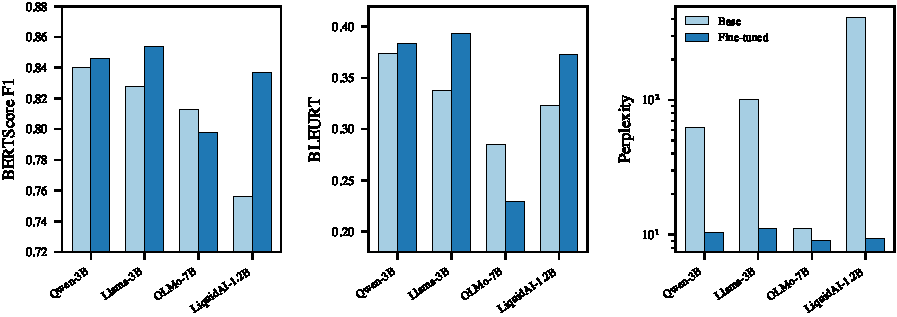
\includegraphics[width=\textwidth]{figures/cross_model_comparison.pdf}
\caption{Base vs.\ fine-tuned comparison across all four models on BERTScore F1, BLEURT, and perplexity (log scale). Fine-tuning improves all metrics for three of four models. OLMo-7B is the exception: perplexity decreases but BERTScore and BLEURT degrade after fine-tuning.}
\label{fig:cross-model}
\end{figure*}

\subsection{Human Evaluation}

Table~\ref{tab:human-eval} presents the blinded human evaluation results (mean $\pm$ std over 369 paired samples). Fine-tuning improves the average rating from $4.37 \pm 1.19$ to $4.71 \pm 0.75$ (+0.34), with the largest gain on naturalness (+0.37). A paired Wilcoxon signed-rank test confirms this improvement is highly significant ($p < 10^{-5}$). GPT-4o-mini scores highest overall ($4.82 \pm 0.62$), though the gap to the fine-tuned model is modest; the fine-tuned model significantly differs from the few-shot baseline ($p < 0.01$). The domain breakdown reveals that task-oriented dialogue (SGD) benefits substantially more from fine-tuning ($+0.45$, $p < 10^{-8}$) than open-domain conversation (WildChat, $+0.21$, $p = 0.12$, n.s.), suggesting that structured intent patterns are easier to learn from limited data.

\begin{table}[h]
\centering
\caption{Human Evaluation (mean $\pm$ std, $n{=}369$, 1--5 Likert)}
\label{tab:human-eval}
\resizebox{\columnwidth}{!}{%
\begin{tabular}{lcccc}
\toprule
\textbf{Condition} & \textbf{Rel.} & \textbf{Coh.} & \textbf{Nat.} & \textbf{Avg.} \\
\midrule
Baseline (Qwen-3B) & 4.34{\scriptsize$\pm$1.23} & 4.34{\scriptsize$\pm$1.25} & 4.44{\scriptsize$\pm$1.29} & 4.37{\scriptsize$\pm$1.19} \\
Fine-tuned (Qwen-3B) & 4.64{\scriptsize$\pm$0.88} & 4.68{\scriptsize$\pm$0.85} & 4.81{\scriptsize$\pm$0.75} & \textbf{4.71}{\scriptsize$\pm$0.75} \\
Zero-shot (GPT-4o-mini) & 4.78{\scriptsize$\pm$0.69} & 4.82{\scriptsize$\pm$0.67} & 4.85{\scriptsize$\pm$0.66} & 4.82{\scriptsize$\pm$0.62} \\
Few-shot (GPT-4o-mini) & 4.77{\scriptsize$\pm$0.75} & 4.80{\scriptsize$\pm$0.72} & 4.83{\scriptsize$\pm$0.76} & 4.80{\scriptsize$\pm$0.72} \\
\midrule
\multicolumn{5}{l}{\textit{Domain breakdown (Avg.):}} \\
\quad SGD only ($n{=}200$) & \multicolumn{2}{l}{Base: 4.50{\scriptsize$\pm$1.06}} & \multicolumn{2}{l}{FT: \textbf{4.95}{\scriptsize$\pm$0.22} ($\Delta{=}{+}0.45^{***}$)} \\
\quad WildChat only ($n{=}169$) & \multicolumn{2}{l}{Base: 4.22{\scriptsize$\pm$1.31}} & \multicolumn{2}{l}{FT: 4.43{\scriptsize$\pm$1.01} ($\Delta{=}{+}0.21^{\text{n.s.}}$)} \\
\bottomrule
\multicolumn{5}{l}{\scriptsize Wilcoxon signed-rank: $^{***}p{<}0.001$; $^{\text{n.s.}}$ not significant ($p{=}0.12$).} \\
\end{tabular}}
\end{table}

\section{Discussion}

Our results demonstrate that QLoRA fine-tuning consistently improves user-turn prediction across three of four model families. The improvements are not limited to fluency: BERTScore and BLEURT gains confirm that fine-tuned models produce semantically more appropriate responses, not merely more probable token sequences. The blinded human evaluation reinforces this finding, with fine-tuning raising the average rating by 0.34 points on a 5-point scale (4.71 vs.\ 4.37).

A notable domain asymmetry emerges from the human evaluation: fine-tuning yields a +0.45 improvement on task-oriented dialogue (SGD) but only +0.21 on open-domain conversation (WildChat). This is consistent with the intuition that structured intent patterns in task-oriented settings are easier to learn from limited data, whereas open-domain user behavior is inherently more diverse and less predictable. The finding suggests that domain-specific fine-tuning may be more effective than training on a general-purpose mixture.

OLMo-7B is the sole model where fine-tuning degrades semantic metrics (BERTScore 0.813$\to$0.798, BLEURT 0.285$\to$0.229) despite improving perplexity (11.1$\to$9.0). This dissociation suggests the model learns to produce more fluent text but loses semantic alignment with the ground truth. A likely explanation is that our ablation was conducted on the 1.2B LiquidAI model, and the resulting configuration may not transfer well to OLMo's larger 7B architecture, which may require a different LoRA rank or learning rate.

The GPT-4o-mini prompt baselines achieve strong results (0.847 BERTScore few-shot) and score highest in human evaluation (4.80--4.82). However, this comparison is asymmetric: GPT-4o-mini is a substantially larger proprietary model that cannot be fine-tuned or conditioned on user-turn data through its API. Importantly, the fine-tuned Llama-3B (a 3B open-source model) surpasses GPT-4o-mini on automated metrics (0.854 BERTScore, 0.393 BLEURT), demonstrating that parameter-efficient fine-tuning of small open models can be competitive with or exceed large proprietary alternatives.

The ablation study reveals that the LoRA scaling factor $\alpha$ is the most impactful hyperparameter, while rank has minimal effect ($r{=}8$ performs comparably to $r{=}64$). This aligns with the hypothesis of Hu et al.~\cite{hu2021lora} that adaptation updates reside on a low intrinsic dimension, and suggests that user-turn behavioral adaptation occupies a particularly compact subspace. Dropout of 0.0 proved optimal, indicating that regularization is unnecessary at this data scale.

The temperature sweep confirms that lower temperatures (0.3) optimize automated metrics for most models, as more deterministic decoding better matches the single ground-truth reference. OLMo again diverges, preferring 0.6, which may reflect its need for higher output diversity to compensate for reduced semantic alignment after fine-tuning.

\textbf{Limitations.} Our study has several constraints. The human evaluation relies on a single rater, precluding inter-rater reliability analysis. The ablation was conducted on the smallest model only; the OLMo regression demonstrates that optimal configurations may not transfer across architectures. All experiments are English-only. Furthermore, our evaluation measures similarity to a single ground-truth user turn, whereas multiple valid continuations exist in practice. Finally, we evaluate single-turn predictions rather than multi-turn rollouts, leaving interactive coherence untested.

\section{Conclusion}

We investigated QLoRA fine-tuning for next user turn prediction across four open-source LLMs ranging from 1.2B to 7B parameters. Training on just 6{,}000 samples yields consistent improvements in fluency and semantic quality for three of four models, with the fine-tuned Llama-3B achieving the best automated scores (0.854 BERTScore, 0.393 BLEURT). A blinded human evaluation of 369 samples confirms gains in relevance, coherence, and naturalness, with task-oriented dialogue benefiting more than open-domain conversation.

From a practical standpoint, QLoRA makes user-turn modeling accessible on a single GPU, and fine-tuned open-source models can match or surpass proprietary API alternatives on automated metrics. The full pipeline, including data processing, training, evaluation, and Docker configuration, is publicly available to support reproducibility.

Future work should address multi-turn rollout evaluation, where generated user turns are fed back into the conversation to assess interactive coherence. Per-model ablation studies could resolve the OLMo regression, and scaling to larger training sets and multilingual data would test generalization further. Finally, preference-based training methods such as DPO could improve user-turn quality beyond what supervised fine-tuning alone achieves.

\section*{Acknowledgment}

\bibliographystyle{IEEEtran}
\bibliography{reference}

\end{document}
